\documentclass[a4paper,12pt]{article}

\usepackage{graphicx}   % For including images
\usepackage{setspace}   % For line spacing
\usepackage{geometry}   % To adjust margins
\usepackage{ragged2e}
\pagestyle{empty} % Remove page numbers
\geometry{margin=1in}   % Set margin size

\title{
  \vspace{-2em} % Adjust the space above the title
  \textbf{CS702- Computing Lab} \\ % Main title
  \large \textbf{ Department of Computer Science and Engg.- NITK Surathkal} \\ % Subtitle
  \vspace{1em} % Space between subtitle and author
  \textbf{ABHIJITH C} \\ % Author
  Roll Number: 242CS003 \\% Roll number
  \textbf{ANAND M K} \\ % Author
  Roll Number: 242CS008 \\% Roll number
}

\date{} % Remove the date

\begin{document}
\maketitle

% Title Page
\begin{titlepage}
\begin{center}

    \vspace*{0.1in}

    {\Huge\bfseries Conversational Used Car Price Predictor\par}
    \vspace{1in}
\end{center}

\section*{Introduction}
\begin{justify}
In today’s world, conversational interfaces are essential for making interactions with technology more easier and more natural. They use innovative technology to chat with users, understand their needs, and provide helpful responses. 
\newline

The latest statistics reveal a significant increase in the demand for used cars. As this market grows, many consumers face the challenge of accurately evaluating car prices due to a need for knowledge and information. This is where price prediction using Machine Learning  becomes significant. 
\newline

The main goal of this project is to develop a conversational interface which will interact with the user to get the necessary parameters for the prediction model. The prediciton model will generate the car price which will be displayed to the user through the interface.
\newline


\end{justify}

\section*{Problem Statement and Objectives}
\begin{justify}
Predicting the price of used cars using Machine Learning model requires large number of features and parameters such as car manufacturer, model, year, mileage and kilometres driven. Traditional methods for evaluating car prices often involve filling out forms.It can be a confusing and less interactive process for consumers to manually input different details which leads to a frustrating user experience. 
\newline

To offer a more user-friendly experience, this project aims to develop a chatbot that integrates with the price prediction model. This interface will guide users through a step-by-step process to collect the necessary car details


\end{justify}

\end{titlepage}

\newpage
\section*{Solution and Different Phases of the Project}
\begin{justify}
\begin{figure}[h]
    \centering
    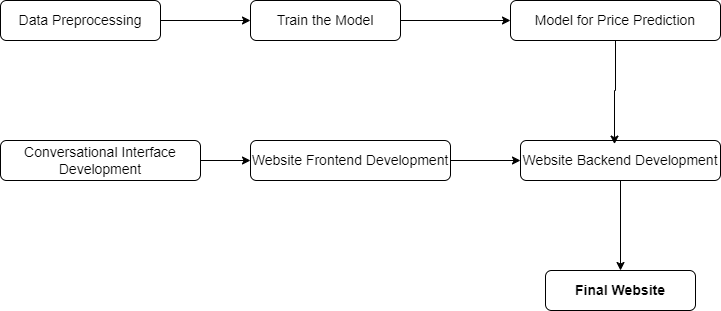
\includegraphics[width=.8\textwidth]{./Flowchart2.png}
    \caption{Solution Flowchart}
    \label{fig:your-label}
\end{figure}
\vspace{\baselineskip} 
\begin{itemize}
\item The first phase of the project is to find an appropriate dataset and perform data preprocessing. Datasets can be accessed from various websites, such as Kaggle. Python libraries, including Pandas and NumPy, can be used for this preprocessing. 

\item The second phase of the project is to train the model. The Scikit-learn library can be used for implementing machine learning regression algorithms.


\item The third phase of the project is to compare the performance of different algorithms using performance metrics such as Mean Absolute Error (MAE) and select the most accurate algorithm. 


\item The fourth phase of the project is to develop the Conversational Interfaces. Open-source frameworks like Rasa can be used to develop the conversational interface, utilizing NLP techniques to process user input, extract intents and entities from the conversation, and generate appropriate replies. 

\item The fifth phase focuses on developing the frontend of the website, which involves designing and implementing the user interface (UI) for the conversational interface. This will include a Chat Interface: A conversational UI where users can interact with the system through natural dialogue. This interface will guide users in providing necessary details about their cars and receiving price predictions. The UI can be implemented using web development tools such as HTML, CSS, JavaScript, and React.js


\item The sixth phase of the project is to develop the backend of the website. This can be implemented using Python frameworks such as Flask or Django.


\item The seventh and final phase of the project involves integrating the frontend and backend through API calls. Following integration, testing will be conducted using various test cases. Finally, documentation for the project will be prepared.
\end{itemize}
\newpage
\section*{Exepected Outcomes}
	\begin{itemize}
		\item The conversational interface will effectively interact with users, guiding them through the process of providing necessary car details in a natural and engaging manner.
		\item A predictive model that provides accurate predictions based on user inputs.
		\item Successful integration of the frontend and backend.

	 \end{itemize}

\section*{Tentative Timeline}
\begin{tabular}{|c|p{7cm}|c|}
\hline
\textbf{PHASE} & \textbf{DESCRIPTION} & \textbf{TIMELINE} \\ \hline
1 & Finalizing project Design \& Module division & September 4 - September 10 \\ \hline
2 & Dataset collection and pre-processing & September 11 - September 18 \\ \hline
3 & Train Model and Compare Algorithm Performance & September 19 - September 30 \\ \hline
5 & Conversational Interface development & October 1 - October 19 \\ \hline
6 & Frontend Development & October 20 - November 4 \\ \hline
7 & Backend Development & November 5 - November 16 \\ \hline
8 & Integration, Testing, and Documentation & November 17 - November 20 \\ \hline
\end{tabular}


\begin{thebibliography}{9}
\bibitem{varshitha2022}
J. Varshitha, K. Jahnavi, and C. Lakshmi, "Prediction Of Used Car Prices Using Artificial Neural Networks And Machine Learning," \textit{2022 International Conference on Computer Communication and Informatics (ICCCI)}, Coimbatore, India, 2022, pp. 1-4, doi: 10.1109/ICCCI54379.2022.9740817.


\bibitem{kathiravan2023}
M. Kathiravan, M. Ramya, S. Jayanthi, V. V. Reddy, L. Ponguru, and N. Bharathiraja, "Predicting the Sale Price of Pre-Owned Vehicles with the Ensemble ML Model," \textit{2023 4th International Conference on Electronics and Sustainable Communication Systems (ICESC)}, Coimbatore, India, 2023, pp. 1793-1797, doi: 10.1109/ICESC57686.2023.10192988.


\end{thebibliography}

\end{justify}

\end{document}
